\documentclass{article}
\usepackage[english]{babel}
\usepackage[utf8]{inputenc}
\usepackage{amsmath}
\usepackage{graphicx}
\usepackage[colorinlistoftodos]{todonotes}

\title{CIS 519 Problem Set 3}

\author{Gabrielle Merritt}


\begin{document}
\maketitle
\part{Problem Set}

\section{Probability decision boundary}

\subsection{Show that decision $\hat{y}$ that minimizes the expected loss equivalent to setting a probability threshold $\theta$ and predicting $ \hat{y} = 0$  if $p1<\theta$ and $\hat{y} = 1$ if $p1 \geq \theta$}
\paragraph{solution}
If we assume the threshold is where Cost of predicting 0 and predicting 1 are equivalent, then we can assume p1 acts a threshold for predicting 1 or 0 
$$cost_0 = 0*p_0 + 10*p_1 $$
$$cost_1 = 5*p_0 + 0*p_1 $$
$$p_1 = \frac{1}{2}p_0 $$  

\subsection{Calculate the threshold}
\paragraph{solution}
$$\theta = p_1 $$ when  $cost_0 = cost_1 $
also 
$$p_1 = 1 - p_0$$
therefore: 
$$ 1 - p_0 = \frac{1}{2}p_0 $$ 
$$ p_0 = \frac{2}{3} $$
$$ \theta = 1 - \frac{2}{3} = \frac{1}{3} $$ 


\section{Double Counting the evidence}
\subsection{What is expected error rate of Naive Bayes only using $X_1$? what if only uses $X_2$}
\paragraph{Error rate only using $X_1$}
\begin{tabular}{l*{2}{c}||r}
$X_1$              & $P(X_1|Y =T)P( Y =T)$ &$P(X_1|Y =F)P( Y =F) $ & $\hat{Y}$ \\
\hline
T & $.5 *.8 $& $.5*.3$  & T   \\
F & $.5* .2$ & $.5 * .7$  &  F  \\
\end{tabular}
\linebreak
$$Expected Error X_1 = .15 +.1 =0.25 $$ 
\paragraph{Error rate only using $X_2$}
\begin{tabular}{l*{2}{c}||r}
$X_2$              & $P(X_2|Y =T)P( Y =T)$&$P(X_2|Y =F)P( Y =F) $ & $\hat{Y}$ \\
\hline
T & $.5 *.5 $& $.5*.1$  & T   \\
F & $.5* .5$ & $.5 *.9$  &  F  \\
\end{tabular}
\linebreak
$$Expected Error X_2 = 0.05 +.25 =0.30 $$ 


\subsection{Show that if naive Bayes uses both attributes $X_1$ and $X_2$ the error rate is 0.235, which is better than the single attribute}
\paragraph{Solution:}
\begin{tabular}{l*{2}{c}||r}
$X_1$ $X_2$             & $P(X_1, X_2|Y =T)P( Y =T)$&$P(X_1, X_2|Y =F)P( Y =F) $ & $\hat{Y}$ \\
\hline
T T & $.5 *.8* .5$ & $.5*.3*.1 $  &  T \\
T F & $.5* .8* .5$ & $.5 *.3*.9$  &  T  \\
F T & $.5* .2* .5$ & $.5 *.7*.1$  &  T  \\
F F & $.5* .2* .5$ & $.5 *.7*.9$  &  F   \\
\end{tabular}
\linebreak
$$Expected Error( X_1, X_2)  = 0.015 +0.135 +0.035+ 0.05 =0.235 $$ 

\subsection{Now suppose that we create new attribute$ X_3$ that is an exact copy of $X_2$. So for every training example, attributes$ X_2 $and $X_3$ have the same value. What is the expected error of naive Bayes now?}
\paragraph{Solution:}
\begin{tabular}{l*{2}{c}||r}
$X_1$ $X_2$ $X_3$   & $P(X_1, X_2|Y =T)P( Y =T)$&$P(X_1, X_2|Y =F)P( Y =F) $ & $\hat{Y}$ \\
\hline
T T T & $.5 *.8*.5 *.5$ & $.5*.3*.1*.1 $   &  T \\
T F F & $.5* .8* .5 *.5$ & $.5 *.3*.9*.9$  &  F  \\
F T T & $.5* .2* .5 *.5$ & $.5 *.7*.1*.1$  &  T  \\
F F F & $.5* .2* .5 *.5$ & $.5 *.7*.9*.9$  &  F   \\
\end{tabular}
\linebreak
$$Expected Error( X_1, X_2,X_3)  = 0.0015 +0.1 +0.0035+ 0.025 =0.13 $$

\subsection{Explain what is happening above}
\paragraph{Solution:}
By adding $X_3 = X_2$ we are skewing the predictions to more heavily relying on $X_2$ to predict our labels 
 
\subsection{Does logistic regression suffer from the same problem}
Yes, logistic regression like Naive Bayes assumes each feature is independent from each other, so if two features like $X_2$ and $X_3$ are dependent the function will be improperly weighted. 

\section{Reject Option}
\subsection{Suppose $p(y = 1|x) = 0.2$. Which decision minimizes the expected loss?}
\paragraph{solution}
$$p(y =0|x) = 1 -p(y =1|x) = .8 $$
$$ Cost \hat{Y_0}  = 0 *p_0 +10*p_1  = 2$$
$$Cost \hat{Y_1} = 10*p_0 + 0 *p_1 = 8 $$ 
$$Cost reject =  3*p_0 +3*p_1  = 2.4 + .6 = 3$$ 
Predicting $\hat{Y_0} $ minimizes loss

\subsection{Now suppose$ p(y = 1|x) = 0.4$. Now which decision minimizes the expected loss?}

$$p(y =0|x) = 1 -p(y =1|x) = .6 $$
$$ Cost \hat{Y_0}  = 0 *0.6 +10*0.4 = 4$$
$$Cost \hat{Y_1} = 10*0.6 + 0 *0.4 = 6 $$ 
$$Cost reject =  3*0.6 +3*0.4  = 1.8 + 1.2 = 3$$ 
Rejecting minimizes loss

\subsection{Show that in cases such as this there will be two thresholds,$\theta{_0}$ and $\theta{_1}$ such that the optimal decision is to predict 0 if $p_1 < \theta{_0}$, reject if $\theta{_0} \leq p_1 \leq \theta{_1}$, and predict 1 if $p_1 > \theta{_1}$}
Again using when the costs are equal to determine threshold 
$$p1 = 1 - p_0$$
$$ 0*p_0 +10p_1 = 3p_0 + 3p_1 = 10p_0 + 0p_1$$
$$p_1 = \frac{3}{7}p_0 $$
$$1-p_0 = \frac{3}{7}p_0 $$ 
$$p_0 = .7 $$
$$\theta{_0} = \frac{3}{7}p_0  = .3 $$
$$\theta{_1} = \frac{7}{3}p_1 = .7 $$

\subsection{what are the threshold for new matrix}
$$p1 = 1 - p_0$$
$$ 0*p_0 +10p_1 = 3p_0 + 3p_1 = 5p_0 + 0p_1$$
$$p_1 = \frac{3}{7}p_0 $$
$$1-p_0 = \frac{3}{7}p_0 $$ 
$$p_0 = . $$
$$\theta{_0} = \frac{3}{7}p_0  = .3 $$
$$\theta{_1} = \frac{3}{2}p_1 = .45$$
\part{Programming}
\subsection{Visualizing hidden nodes }

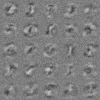
\includegraphics[width = \linewidth]{test1.jpg}
 Reg lambda = .014 
 \linebreak
 numEpoch = 100 
 \linebreak
 lambda = .9 
 \linebreak
 epislon  = .9
 \linebreak
 Training accuracy ~ 86% 

\end{document}
